\documentclass[12pt]{article}
\usepackage[T1]{fontenc}
\usepackage[slovak]{babel}
\usepackage{mathptmx}

\usepackage{caption}
\usepackage{subcaption}
\usepackage{indentfirst}


\usepackage[width=\textwidth]{svg}

\usepackage[a4paper,left=35mm,
                    right=25mm,
                    top=25mm,
                    bottom=25mm]{geometry}

\linespread{1.5}   % 1.5 riadkovanie

\AddToHook{cmd/section/before}{\clearpage}

\def\nazovprace{Botanica - simulátor rastlín na báze celulárnych automatov}
\def\autori{František Knapec, Michael Sklenka, Marek Beňo}

\begin{document}

\begin{titlepage}
	\setlength{\parindent}{0pt}

	\begin{center}
		Gymnázium \\
		Veľká okružná 22, 010 01 Žilina

		\vspace{7cm}
		\Huge \nazovprace

		\vspace{1.13cm}
		\Large Stredoškolská odborná činnosť

		\vspace{2.12cm}
		\normalsize Č. odboru: 11
	\end{center}

	\vfill

	\begin{minipage}{0.75\textwidth}
		Riešitelia: \autori \par
		Ročník štúdia: 4.
	\end{minipage}
	\hfill
	\begin{minipage}{0.23\textwidth}
		\hfil % basically align right
		\begin{tabular}{rc}
			Mesto: & Žilina \\
			Rok:   & 2025
		\end{tabular}
	\end{minipage}
\end{titlepage}

\begin{titlepage}
	\setlength{\parindent}{0pt}

	\begin{center}
		Gymnázium \\
		Veľká okružná 22, 010 01 Žilina

		\vspace{7cm}
		\Huge \nazovprace

		\vspace{1.13cm}
		\Large Stredoškolská odborná činnosť

		\vspace{2.12cm}
		\normalsize Č. odboru: 11
	\end{center}

	\vfill

	\begin{minipage}{0.75\textwidth}
		Riešitelia: \autori \par
		Ročník štúdia: 4. \par
		Školiteľ: Ing. Tomáš Milet, PhD.\par

	\end{minipage}
	\hfill
	\begin{minipage}{0.23\textwidth}
		\hfil % basically align right
		\begin{tabular}{rc}
			\\ \\
			Mesto: & Žilina \\
			Rok:   & 2025
		\end{tabular}
	\end{minipage}
\end{titlepage}

% zapocitaj strany
\setcounter{page}{3}


\thispagestyle{empty}

\null
\vfill

\noindent
\textbf{Čestné vyhlásenie:}

Prehlasujeme, že sme prácu na tému
\nazovprace \space
vypracovali samostatne s~použitím literatúry uvedenej v~zozname použitej literatúry.
Zároveň prehlasujeme, že sme predloženú písomnú prácu neprihlásili a ani neprezentovali
v žiadnej inej súťaži, ktorá je pod gestorstvom MŠMVVaŠ SR. Sme si vedomí zákonných dôsledkov,
ak v~nej uvedené údaje nie sú pravdivé.

\vspace{5cm}

\newpage


%
% Poďakovanie (nepovinné)
%

% \thispagestyle{empty}
% 
% \null
% \vfill
% 
% \noindent
% \textbf{Poďakovanie}
% 
% \noindent
% Toto je poďakovanie
% 
% \vspace{8cm}
% \newpage


\thispagestyle{empty}
\tableofcontents

%
% The work :)
%

\section*{Úvod}
\addcontentsline{toc}{section}{Úvod}

Väčšina hier s~otvoreným procedurálne generovaným svetom vníma rastliny iba ako
jednoduché prvky pre skrášlenie sveta. Pre veľa hier je tento prístup ideálny,
avšak ním prichádzajú o pestrosť a zaujímavosť, ktorú ponúkajú simulácie.
Simulovanými rastlinami môžu benefitovať hlavne hry o prežitie a hry, v ktorých
môže hráč upravovať svet.

Mimo vizuálne pekného prostredia ponúkajú simulované rastliny aj možnosti
mnohých unikátnych mechaník ako napríklad možnosť geneticky
modifikovať rastliny, čím by hráč mohol napríklad zvýšiť produkciu svojej záhrady
v hrách o prežitie.

Táto práca sa zaoberá aplikáciou demonštrujúcou jednoduchý algoritmus
pridávajúci rastlinám možnosť reagovať na okolité prostredie. Aplikácia
simuluje a vykresľuje rastliny v procedurálne generovanej časti sveta.
Rastliny reagujú na množstvo látok (dusík, draslík a fosfor) v zemine,
množstva vody a svetla pomocou ich genómu.

Najprv sú vysvetlené základné pojmy, algoritmy a praktiky používané pri tvorení
herného sveta. Následne je predstavená aplikácia, ktorá demonštruje algoritmus
pre jednoduché spestrenie rastlín vo svete. Záver práce sa venuje možným
zlepšeniam aplikácie a ďalším využitiam simulovania rastlín v hrách
s otvoreným svetom.


\section{Problematika a prehľad literatúry}

Táto práca sa zaoberá implementovaním rastlín do digitálnej podoby a následným
simulovaním ich správania relatívne k podmienkam, v ktorých sa nachádzajú,
ako aj k iným rastlinám v ich okolí. Jej súčasťou je aj vyobrazenie
rastlín v trojrozmernom priestore. Pôjde aj o schopnosť dlhodobého
pozorovania ekosystému naprieč časom.

Ľudia k problému tvorenia digitálnych rastlín pristupovali rôznymi spôsobmi,
avšak väčšina z nich len realistické rastliny vykresľovala, pozri napríklad
známy príklad\break L-systémov (Prusinkiewicz, Hanan, 2013). % cite
Tento systém je založený na opisovaní štruktúry rastlín
sériou pravidiel, ako je napr. otočenie, vytvorenie úsečky alebo
vrátenie sa na určitú pozíciu. Ďalej sa štruktúra zdokonaľuje za pomoci
algoritmu, ktorý nahrádza časti jej série pravidiel za iné, dopredu určené
a detailnejšie série. Tento postup dokáže vytvoriť celkom realistické rastliny
ako je znázornené na obr. \ref{obr:priklad l-systemu}.

\begin{figure}[ht]
	\centering
	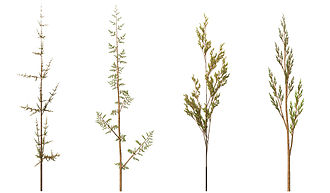
\includegraphics[width=0.5\textwidth]{res/Fractal_weeds.png}
	\caption{Príklad tráv vygenerovaných s použitím L-systému v 3D}

	\footnotesize (zdroj: https://en.wikipedia.org/wiki/L-system)

	\label{obr:priklad l-systemu}
\end{figure}

Toto riešenie a jemu podobné dané rastliny len vytvárajú, no našim cieľom
je aj simulovať ich život.


\subsection{Spôsoby simulovania rastlín}

Kvôli samotnej simulácii vzniklo viacero metód simulovania s vlastnými kladmi,
ale aj zápormi. Medzi takéto metódy patria:

\begin{itemize}
	\item \textbf{Fyzikálne založené modelovanie} využívajúce body prepojené
	      pružnými štruktúrami, na ktoré pôsobia rôzne sily. Aj keď realistické,
	      modelovanie neumožňuje rastliny tvoriť, iba simulovať.
	\item \textbf{Simulácia pomocou strojového učenia}
	      využíva štatistické
	      algoritmy, pomocou ktorých sa počítač dokáže počas tréningu učiť vzťahy medzi
	      vstupmi a výstupmi.
	\item \textbf{Celulárne automaty} (ďalej CA)
	      je názov pre matematický model a nástroj pre simuláciu. Jedná sa
	      o starší koncept, ktorý obsahuje štvorcovú sieť so „zafarbenými“
	      políčkami. Každá farba predstavuje určitý stav, ktorý má špecifické správanie
	      závisiace od okolitých políčok.
\end{itemize}

Fyzikálne založené modelovanie, aj keď mocné, vyžaduje, aby rastliny boli
vygenerované dopredu, pred začatím simulácie a po jej spustení nie sú tieto
rastliny schopné sa ďalej vyvíjať. Navyše spôsob vyžaduje fyzikálne založenú
simuláciu, ktorá je príliš komplikovaná pre túto prácu.

Na druhej strane, strojové učenie sa stáva čím ďalej tým využívanejšie pre
riešenie všetkých možných problémov. Avšak tento spôsob je náročný na čas
a výpočtovú techniku.

A napokon celulárne automaty ponúkajú jednoduchosť a možnosť ich ľahko
modifikovať, čo otvára pole rôznorodých využití. (Gutowitz, 1991)
Práve tieto výhody nás presvedčili a simulácia
v tejto práci sa zakladá na princípe celulárnych automatoch.

\subsection{Celulárne automaty}

CA sa skladá z týchto základných častí: mriežka (často štvorcová sieť)
a bunky tejto mriežky, ktoré majú vlastný stav. Každý stav obsahuje
určité pravidlá, ktoré zapríčiňujú správanie buniek, a tým celého systému.
Tieto pravidlá sa aplikujú každú generáciu, každé simulačné kolo.
Vďaka týmto vlastnostiam sú CA systém, ktorý je jednoduché prispôsobiť ktorýmkoľvek
požiadavkám.

Klasickým príkladom takéhoto systému je Conwayova hra života (Adamatzky, 2010).
V tejto hre nadobúda každá bunka štvorcovej siete jednu z dvoch hodnôt:
Buď je bunka živá alebo mŕtva. Conwayova hra života má nasledovné pravidlá:

\begin{enumerate}
	\item Každá živá bunka s menej ako dvomi živými susedmi umrie.
	\item Každá živá bunka s dvomi alebo tromi živými susedmi prežije.
	\item Každá živá bunka s viac ako tromi živými susedmi umrie.
	\item Každá mŕtva bunka s presne tromi živými susedmi ožije.
\end{enumerate}

V hre života sa nachádza veľa stabilných konfigurácií (glidery, továrne,
oscilátory, atď.). Na obr. \ref{obr:conwayova hra zivota} je znázornená
pohyblivá štruktúra (červená), ktorá
za sebou zanecháva továrne (zelená) produkujúce glidery (modrá),
jednoduché pohybujúce sa štruktúry.
Vďaka týmto štruktúram je Conwayova hra života Turingovo kompletná (môže
simulovať hocijaký počítač, čiže aj sama seba\footnote
{Life in life - https://www.youtube.com/watch?v=xP5-iIeKXE8}).

\begin{figure}[ht]
	\centering
	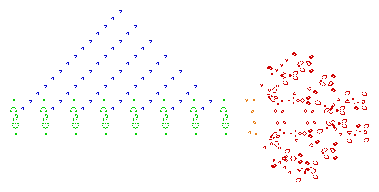
\includegraphics[width=0.9\textwidth]{res/Conways_game_of_life_breeder.png}
	\caption{Rôzne typy štruktúr v CA.}
	\label{obr:conwayova hra zivota}
\end{figure}

\subsubsection{Príklady CA zamerané na simuláciu rastlín}

Práca (Winarno, Prima, Afifah, 2016) sa zameriava na
korene rastlín a dopad premenných ako napr. živiny v pôde, voda a prekážky
v raste. Jedná sa o prácu, ktorá je viac zameraná na matematický popis rastu koreňov,
avšak my sme rast koreňov simulovali genetikou.

Práca (Bandini, Pavesi, 2004) sa zameriava na 2D simuláciu heterogénnej populácie
rastlín, orientuje sa na konkurenciu medzi druhmi, rýchlosť rastu a interakcie
s prostredím.

\section{Ciele práce}

Cieľom tejto práce je vytvorenie aplikácie schopnej tvorenia a simulácie
pseudo-rea\-listických rastlín v trojrozmernej mriežke pomocou celulárnych
automatov a implementovanej genetiky.
Tieto rastliny by mali byť schopné reagovať na prostredie v reálnom čase
a adaptovať svoje správanie, tvar a iné charakteristiky v závislosti
od podmienok, v ktorých sa nachádzajú.

Výsledkom tejto práce je softvér, Botanica, ktorý umožňuje pozorovanie
správania a vývinu simulovaných rastlín vďaka schopnostiam:

\begin{enumerate}
	\item generovať časť 3D voxelového sveta za pomoci Perlinovho šumu,
	\item simulovať rastliny vo vytvorenom prostredí pomocou vlastného
	      algoritmu inšpirovaného celulárnymi automatmi,
	\item vykresľovať túto simuláciu za pomoci grafického API OpenGL.
\end{enumerate}

Veríme, že metódy využité v Botanice sú využiteľné ako na tvorenie dynamického
a nerepetetivného prostredia vo videohrách, tak aj na viac vedecké účely
ako pozorovanie správania rastlín vo virtuálne vytvorených podmienkach
a ich ideálne charakteristiky za daných podmienok.


\section{Aplikácia (Materiál a metodika)}

Na realizovanie algoritmu sme vyvinuli jednoduchú aplikáciu, ktorá má
potrebné prostriedky na demonštráciu všetkých aspektov tohto algoritmu.
Aplikácia umožňuje vizualizáciu rastu rastlín na základe celulárnych automatov
a poskytuje možnosť meniť parametre simulácie na dosiahnutie ideálneho vzhľadu
rastlín.

\subsection{Svet} \label{subsec:svet}

Svet aplikácie pozostáva z mriežky buniek o rozmeroch 32x32x32 voxelov.
Voxel predstavuje základnú jednotku, kocku veľkosti 1x1x1, pri zobrazovaní v priestore.
Každý voxel nadobúda určitý stav. Môže sa jednať o časti rastlín (stonka, list,
koreň alebo ovocie), ale aj o časti terénu (vzduch, voda, pôda).

\subsubsection{Perlinov šum}

Na tvorbu terénu, ktorý nie je len plochá rovina, ale obsahuje aj kopce a údolia,
sa využíva funkcia zvaná Perlinov šum.
Perlinov šum je spôsob generovania plynule sa meniacich náhodných
hodnôt, ktoré sa dajú skvele využiť na generovanie realistického terénu.
Algoritmus jeho generovania je znázornený na obr. \ref{obr:perlinov sum}.

V určitých miestach sa vytvoria modré vektory s náhodným smerom.
Z červených bodov, ku ktorým chceme pripísať hodnoty,
sa vytvoria zelené vektory smerujúce k modrým.
Z modrého a zeleného vektoru sa vytvorí skalárny súčin, ktorý sa následne
pripíše prislúchajúcemu červenému bodu.

\begin{figure}[ht]
	\centering
	\captionsetup{justification=centering}
	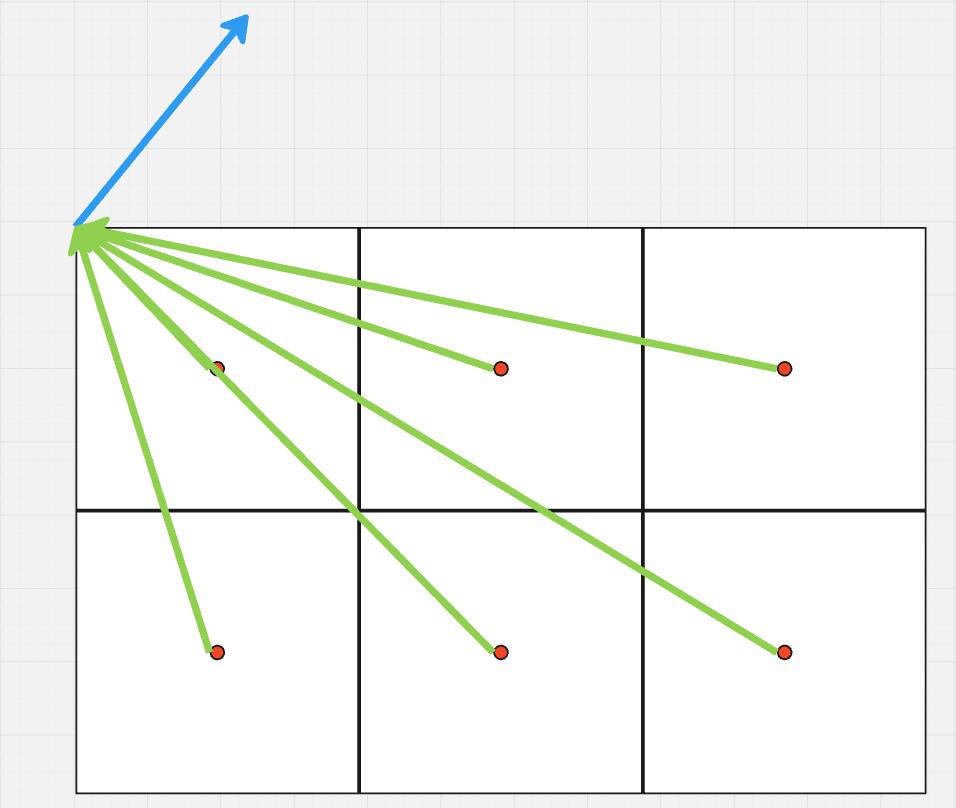
\includegraphics[width=0.5\textwidth]{res/prelinov_sum.png}
	\caption{Znázornenie generovania Perlinovho šumu za pomoci 1 náhodného
		vektoru pre 6 buniek.}
	\label{obr:perlinov sum}
\end{figure}

Väčšinou sa hodnoty nepočítajú len pre jeden náhodný vektor,
ale pre viacero (najčastejšie 4 najbližšie) a hodnoty ich skalárnych
súčinov sa priemerujú. Využíva sa aj viacero oktáv, iterácií algoritmu.
Každá oktáva využíva viac náhodných vektorov ako predchádzajúca,
vďaka ktorým ovplyvňuje bunky menej ako predchádzajúca oktáva.
Často sa hodnoty týchto bodov znázorňujú v dvojfarebnej škále,
ako je vidieť na obrázku~\ref{obr:perlinov sum textura}.

\begin{figure}[ht]
	\centering
	
\includegraphics[width=0.4\textwidth]{res/perlinov_sum_textura.png}
	\caption{Textúra Perlinovho šumu.}
	\footnotesize (zdroj: https://en.wikipedia.org/wiki/Perlin\_noise)zameriava 
	\label{obr:perlinov sum textura}
\end{figure}

Naša aplikácia vďaka jej obmedzenej veľkosti využíva 4 vektory umiestnené
na rohoch simulácie a iba 1 oktávu.

\subsubsection{Tvorenie terénu}

Tvorenie terénu sa začne vytvorením Perlinovho šumu, poďla ktorého sa určí výška terénu.
Pre každú dvojicu súradníc X, Z sa vytvorí hodnota Perlinovho šumu, ktorá určí
výšku terénu v danom bode. Všetky voxely pod touto hodnotou budú pôda, inak
sa bude jednať o voxel vzduchu.

Následne sa určí výška hladiny vody a všetky voxely vzduchu pod touto hladinou
sa premenia vodu.

\begin{figure}[ht]
	\centering
	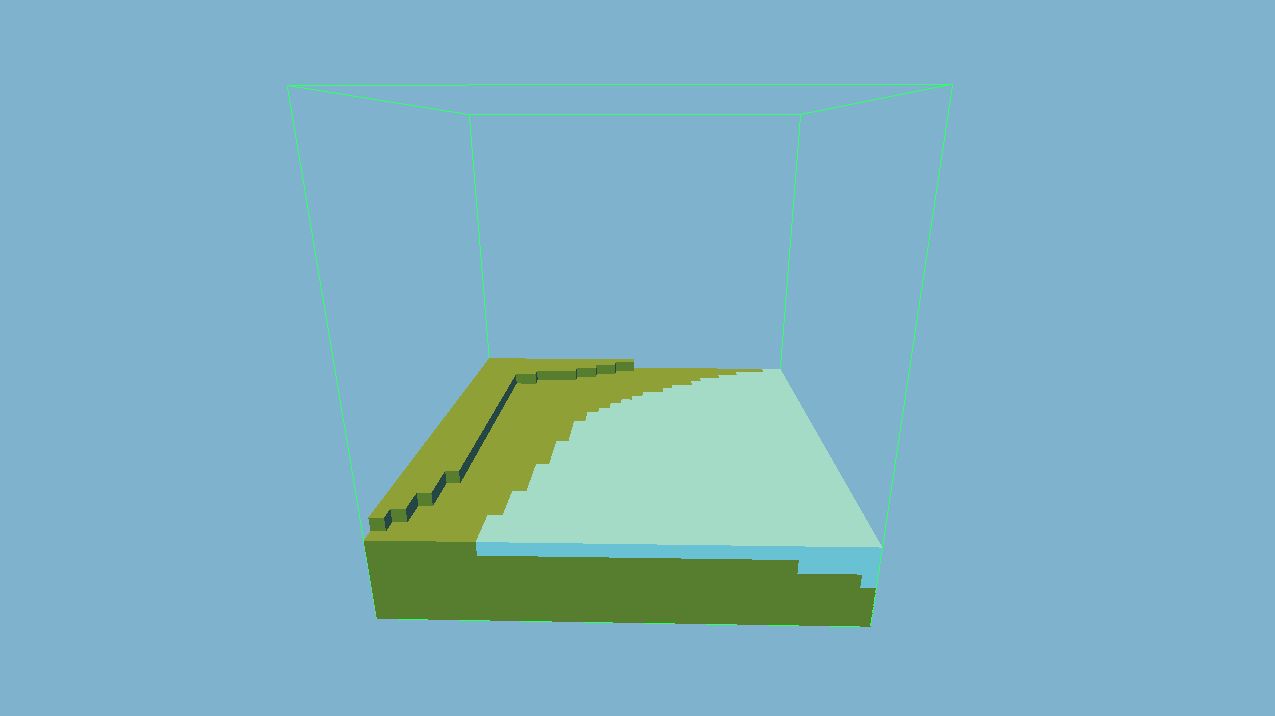
\includegraphics[width=0.9\textwidth]{res/terrain.png}
	\caption{Terén vygenerovaný touto technikou. (voda - modrá, pôda - zelená)}
\end{figure}

\newpage
\subsubsection{Živiny}

Simulácia obsahuje živiny, vodu a vzduch, ktoré rastlina potrebuje pre rast a prežitie.
Voda a vzduch sú zastúpené v podobe ich voxelov. Pôda obsahuje vodu a živiny.
Každá živina napomáha rôznym procesom rastliny, ako napríklad fotosyntetizovať,
čerpať vodu alebo získavať viac živín. Ich nadbytok podporuje rast rastlín
a ich nedostatok tento rast spomaľuje. To pridáva ako na komplexnosti,
tak na realizme a dovoľuje nám získať rôzne typy rastlín, podľa toho,
ku ktorým živinám majú alebo nemajú prístup. Napríklad, ak rastlina nemá dostatok dusíka
potrebného na fotosyntézu, musí tento nedostatok kompenzovať viacerými listami, inak zhynie.

Živiny sú 3: dusík, draslík a fosfor; pričom sme sa snažili o to, aby napomáhali
realistickým procesom, ktoré tieto prvky vyžadujú.
Draslík je nápomocný pri absorpcii vody, takže ak má rastlina nadbytok draslíka,
efektívnejšie získava vodu. Využitie dusíka je široké, ale v simulátore
je jeho funkcia obmedzená len na zlepšenie fotosyntézy, keďže je hlavnou
zložkou chlorofylu. Fosfor je rovnako ako dusík dôležitý v rôznych častiach.
V simulátore je zameraný na absorpciu živín.

\newpage
\subsection{Rastliny}

Rastliny sú v tomto simulátore objekty so spoločnou triedou. Trieda je
predloha premenných a špeciálnych funkcií zvaných metód. Takáto šablóna nám umožňuje
jednoducho a usporiadane tvoriť rastliny, keďže nemusíme písať kód pre každú rastlinu
osobitne.

\begin{figure}[ht]
	\centering
	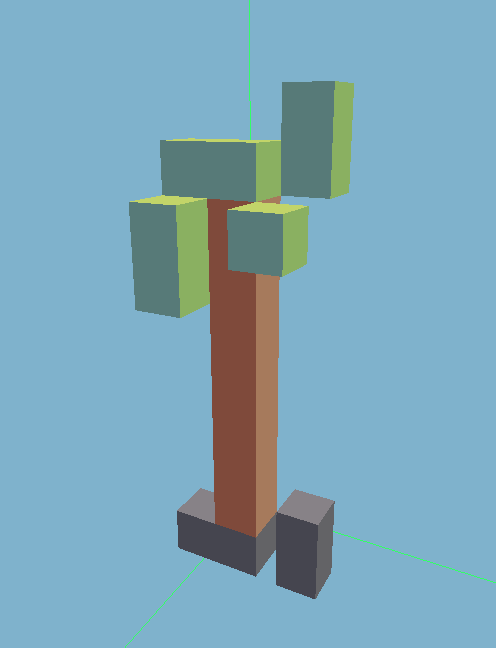
\includegraphics[width=0.5\textwidth]{res/plant.png}
	\caption{Foto rastliny z našej simulácie.}
\end{figure}

\subsubsection{Premenné v rastlinách}

Rastliny majú viacero premenných. Ich hlavnou úlohou je opísať stav rastliny.
Patria medzi ne údaje o získaných živinách, zoznam pozícií všetkých buniek rastliny
a jej gény. V premenných taktiež máme aj bonusy pre živiny.
Hovoria nám o nadbytku alebo nedostatku živín. Bonusy sú rozobrané v kapitole ,,Živiny''.

\newpage
\subsubsection{Voxely rastlín}

Existujú 4 typy voxelov rastlín, kde každý plní vlastnú úlohu.

\begin{itemize}
	\item \textbf{Koreň} má za úlohu rastline získať živiny a vodu. To dosahuje
	odoberaním týchto živín z okolitých voxelov. Môže vzniknúť iba na
	miestach, kde je pôda.

	\item \textbf{List} má za úlohu zbierať slnečnú energiu. To dosiahne tým, že
	skontroluje, či políčka nad ním sú vzduch.

	\item \textbf{Stonka} uskladňuje živiny pre rastlinu a rastie iba zvislo.
	
	\item \textbf{Ovocie} tvorí nové rastliny s pôvodným genetickým kódom,
	ktorý trochu zmutuje. Na pár kôl nahrádza 1 list, ktorý sa po premene
	ovocia na novú rastliny znova zmení na list.
\end{itemize} 

\subsubsection{Genetika a rast}

Na základe genetiky rastliny rozhodujú, aké časti majú rásť (listy, stonka, \dots).
V~prípade listov a koreňov existujú gény určujúce, akým smerom majú rásť.
Takže máme 3 gény: čo má rásť, kde majú rásť korene a kde majú rásť listy.
Gén ,,čo má rásť'' je zoznam so 4 číslami. Sú 4, pretože sú 4 typy buniek,
ktoré môže rastlina rásť. Čísla v týchto zoznamoch označujú,
ako veľmi chce daná rastlina v danej časti rásť. Ak má rastlina hodnotu génu
označujúceho stonku 2 a koreň 10, bude daná rastlina chcieť rásť v koreni
5-krát viac ako v stonke.

O tom, v ktorej časti bude rastlina rásť, rozhoduje náhoda. Keď sa vrátime
k nášmu príkladu, generátor vygeneruje náhodné číslo od 1 do 12, keďže súčet hodnôt
našich génov je $2 + 10 = 12$. Ak bude vygenerované číslo menšie alebo rovné 2,
vyrastie stonka. Ak bude vygenerované číslo väčšie ako 2 vyrastie koreň.

Gény „kde majú rásť korene“ a „kde majú rásť listy“ sú rovnaké,
len ako ich názov napovedá, jeden sa zaoberá koreňmi a druhý listami.
Sú to listy s 26 číslami. Ich hodnôt je 26, pretože bunka má
v trojrozmernom priestore 26 susedov, ak rátame aj diagonály.
Zvyšok funguje rovnako ako gén „čo má rásť“, takže čísla označujú
pravdepodobnosť rastu do daného smeru. Ak sa tieto 2 gény zavolajú, vyberie
sa náhodná bunka (list alebo koreň podľa toho, ktorý gén sa zavolá).
Ak sa bunka nemôže rozrásť do vybraného smeru, tak sa vyberie iná bunka.

\subsection{Algoritmus}

Simulácia postupuje v časových krokoch.
Za každý krok sa vykonajú určité akcie. Tieto akcie slúžia na beh
simulácie a starajú sa o udalosti, ako rast rastlín, ich vznik, smrť atď.
Vďaka tomu možno algoritmus rozdeliť do nasledujúcich častí.

\begin{figure}[ht]
	\centering
	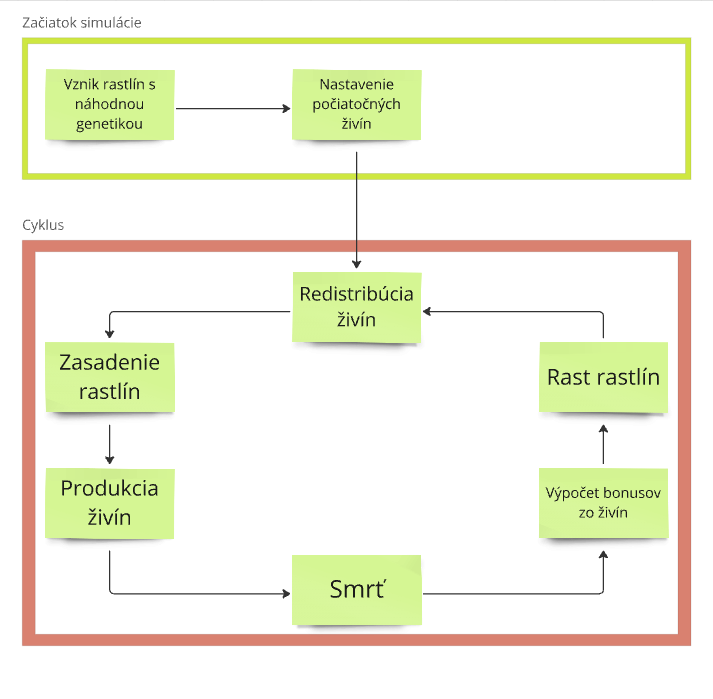
\includegraphics[width=0.7\textwidth]{res/diagram_algoritmu.png}
	\caption{Diagram algoritmu.}
\end{figure}

\subsubsection{Vznik rastlín}

Vznik rastlín je jediná časť algoritmu, ktorá nebeží v krokoch, ale iba raz, a to na začiatku
simulácie. Po vytvorení terénu sa vyberie náhodný voxel pôdy na povrchu, a tam vznikne rastlina.
Počiatočné tvorenie rastlín sa dá opakovať viackrát podľa potreby užívateľa.
Takéto rastliny sa skladajú z 1 koreňa, 1 stonky a 1 listu.
Ich genetika je náhodná, keďže ju nemôžu dediť z materských rastlín, ktoré
neexistujú.

\subsubsection{Redistribúcia živín}

Redistribúcia živín je prvá akcia, ktorá sa vykonáva v každom kroku simulácie. Živiny sú
ukladané v zozname, ktorý drží informácie o ich počte.
V tomto bode je zoznam živín obnovený na hodnoty stanovené v nastaveniach simulácie.
Toto umožňuje rastlinám znovu brať živiny v novom cykle.

\subsubsection{Zasadenie rastlín}

Ak má rastlina ovocie, ktoré existuje po určitú dobu, tak sa z neho stane nová
rastlina. Rozdiel vo vzniku a zasadení je, že genetický kód nie je
vygenerovaný náhodne, ale je zdedený z materskej rastliny,
pričom jedna hodnota náhodne zmutuje, teda sa zmení.

\subsubsection{Produkcia živín}

V tejto fáze rastlina získava živiny vďaka svojim bunkám, konkrétne listom
a koreňom. Pre každý list sa skontrolujú bunky horizontálne nad listom.
Podľa počtu buniek predstavujúcich vzduch, list produkuje svetlo.
Korene zase skontrolujú bunky v ich susedstve podľa čoho generujú živiny a vodu.
Koľko živín z okolitých buniek dokážu listy a korene dostať,
je určené ich počtom v pôde. Maximálny počet živín, ktoré dokáže bunka získať je stanovený
konštantou a bonusom vypočítaným zo živín. Naďalej stonka uskladňuje živiny, takže
rastlina nemôže skonzumovať viac ako jej stonka dovoľuje.

Napríklad rastlina potrebuje fosfor a má koreň s 5 okolitými bunkami,
pričom každá obsahuje 15 jednotiek fosforu. Konštanta produkcie je 10,
a bonus pre fosfor je 1.2, čo koreňu povolí zobrať z každej okolitej bunky až 12
jednotiek fosforu. To predstavuje dokopy 60 jednotiek, ktoré dokáže daný koreň získať.
Avšak kapacita stoniek našej rastliny je len 50, takže náš koreň nakoniec
vyprodukuje len 50 jednotiek fosforu.

\subsubsection{Smrť}

Ak má rastlina nedostatok živín, zomrie. Koľko živín rastlina
potrebuje na prežitie je odvodené od jej veľkosti, čiže počtu jej voxelov
a ceny za voxel.

Ako príklad pozorujme rastlinu s 10 bunkami, cenou za voxel 5 a 45 jednotkami živín.
Cenu za prežitie dostaneme vynásobením počtu buniek rastliny a ceny za voxel
($10 * 5 = 50$). Keďže pozorovaná rastlina vyžaduje na prežitie 50 jednotiek živín, ale má
len 45, zomrie na ich nedostatok.

\subsubsection{Bonusy živín}

Bonusy sa odvíjajú od veľkosti rastliny a špeciálnej konštanty. Ovplyvňujú, koľko
živín dokáže rastlina získať.

\subsection{Vykresľovanie}

Aby simulácia života rastlín bola viac než čísla uložené v súbore, je simulovaný svet
vykresľovaný na obrazovku. Vykresľovanie, v počítačovej grafike bežne označované
ako renderovanie, je prevedené na grafickú kartu.
Procesor má tak viac času venovať sa simulácii. Na renderovaie bolo vybrané
grafické API OpenGL pre jeho jednoduchosť a kompatibilitu medzi operačnými
systémami.

Ako už bolo spomenuté v časti \ref{subsec:svet}, svet je zložený z malých
kociek (voxelov) v sieti 32x32x32. Voxely môžu byť tvorené rôznymi materiálmi,
čo je symbolizované číselnou hodnotou pre každý jeden z nich. Tieto
hodnoty sú po každej zmene sveta nahrané na grafickú kartu pomocou OpenGL.

Grafická karta následne vygeneruje sieť vrcholov s farebnými a
polohovými hodnotami, ktoré sú následne každú snímku vykreslené na obrazovku.

\subsubsection{Tvorenie vrcholov z voxelových dát sveta}

Grafické karty spracovávajú dáta paralelne,
čo im umožňuje ,,prehrýzť'' sa obrovským množstvom dát za okamih.
Je to niečo, na čo treba myslieť pri programovaní compute shaderov
(výpočtových programov). Program na grafickej karte sa nazýva shader.

Shader je spustený niekoľkokrát, raz pre každý voxel. Jeho výstupom je
neprerušená sieť vrcholov, ktoré sú následne zaslané na renderovanie.
To je dosiahnuté globálnym atomickým počítadlom.\footnote
{Atomické počítadlo je číslo, ktoré môže zvýšiť iba jeden program naraz. Táto
	vlastnosť zabraňuje prepisovaniu už zapísaných dát.}

Dáta sú shaderu poslané v jednom veľkom bloku pamäti, čiže shader potrebuje
vedieť, kde sa jemu priradený voxel v tejto pamäti nachádza. Preto má každá
invokácia (každý spustený shader) priradené poradové číslo, ktoré
je použité ako index voxelu v pamäti, z ktorej je vytiahnutá nielen
hodnota jemu priradenému voxelu, ale aj každého susedného voxelu. Tie sú
následne využité na tvorenie stien
(obr. \ref{obr:diagram algoritmu generujuceho vertexy}).

\begin{figure}[ht]
	\centering
	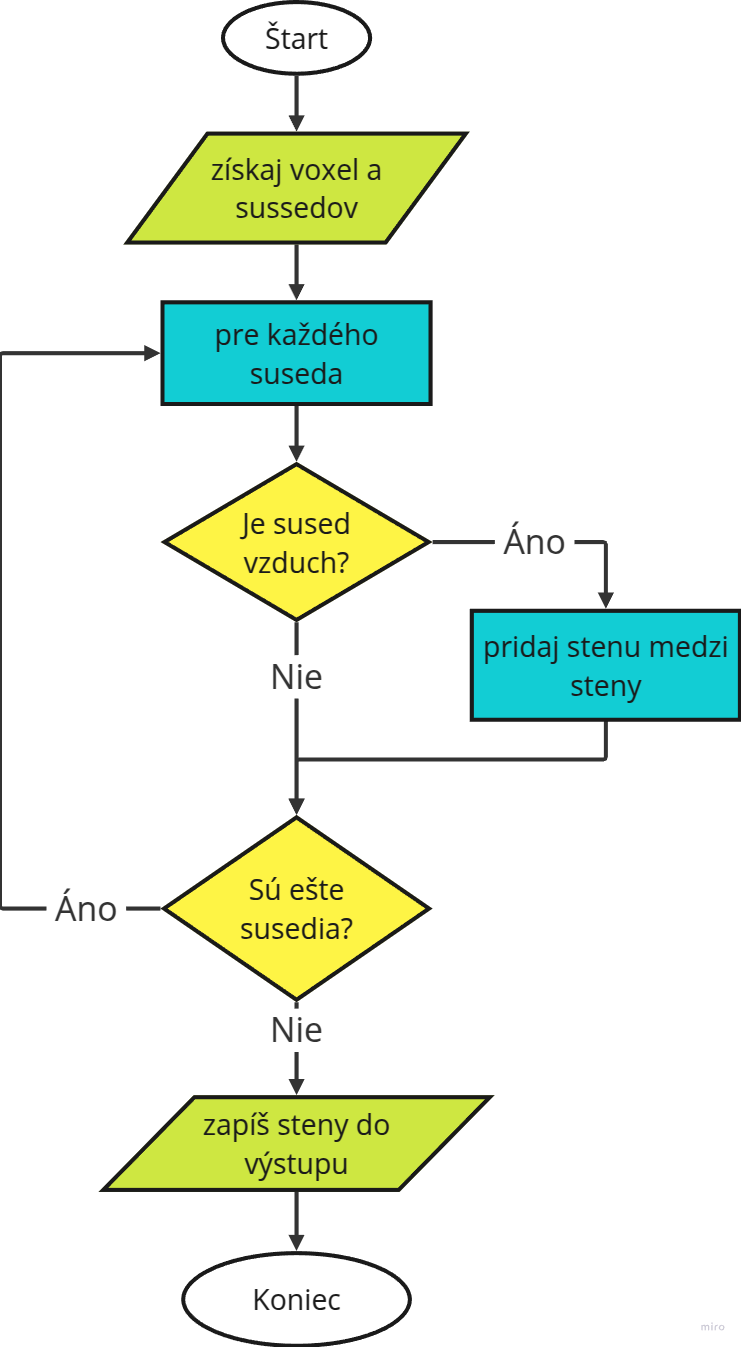
\includegraphics[height=10cm]{res/diagram_generovanie_voxelov.png}
	\caption{Znázornenie algoritmu generujúceho steny (4 vrcholy) okolo priradeného voxelu.}
	\label{obr:diagram algoritmu generujuceho vertexy}
\end{figure}

\subsubsection{Vykresľovanie vygenerovaných dát}

Keď sú dáta vygenerované, nie je zložité ich vykresliť pomocou jednoduchého
programu pozostávajúceho z dvoch častí:

\begin{itemize}
	\item \textbf{vertex shader}, počíta, otáča a posúva body pomocou dát kamery,
	      premieta 3D body na 2D obrazovku,
	\item \textbf{fragment shader}, vyfarbuje trojuholníky tvorené vrcholmi.
\end{itemize}


\section{Výsledky práce a diskusia}

Vytvorená aplikácia Botanica demonštruje možnosť simulácie rastu rastlín
v trojrozmernom prostredí pomocou celulárnych automatov a genetického kódu.
Implementácia zahŕňa: generovanie terénu pomocou Perlinovho šumu, ktorý vytvára
realisticky vyzerajúce prostredie s variabilnou výškou a rozložením živín;
dynamické rastliny, ktoré reagujú na podmienky prostredia a menia svoj rast
na základe genetického kódu a dostupnosti živín; algoritmus rastu, ktorý
zabezpečuje prirodzenú redistribúciu živín, fotosyntézu a rozmnožovanie;
grafickú reprezentáciu založenú na voxelovom engine s renderovaním cez OpenGL,
čo umožňuje vizuálne sledovanie simulovaných procesov. Aplikácia splnila
stanovené ciele. Simulované rastliny vykazujú rôzne formy rastu na základe
ich genetického kódu a podmienok prostredia.

\begin{figure}[ht]
	\centering
	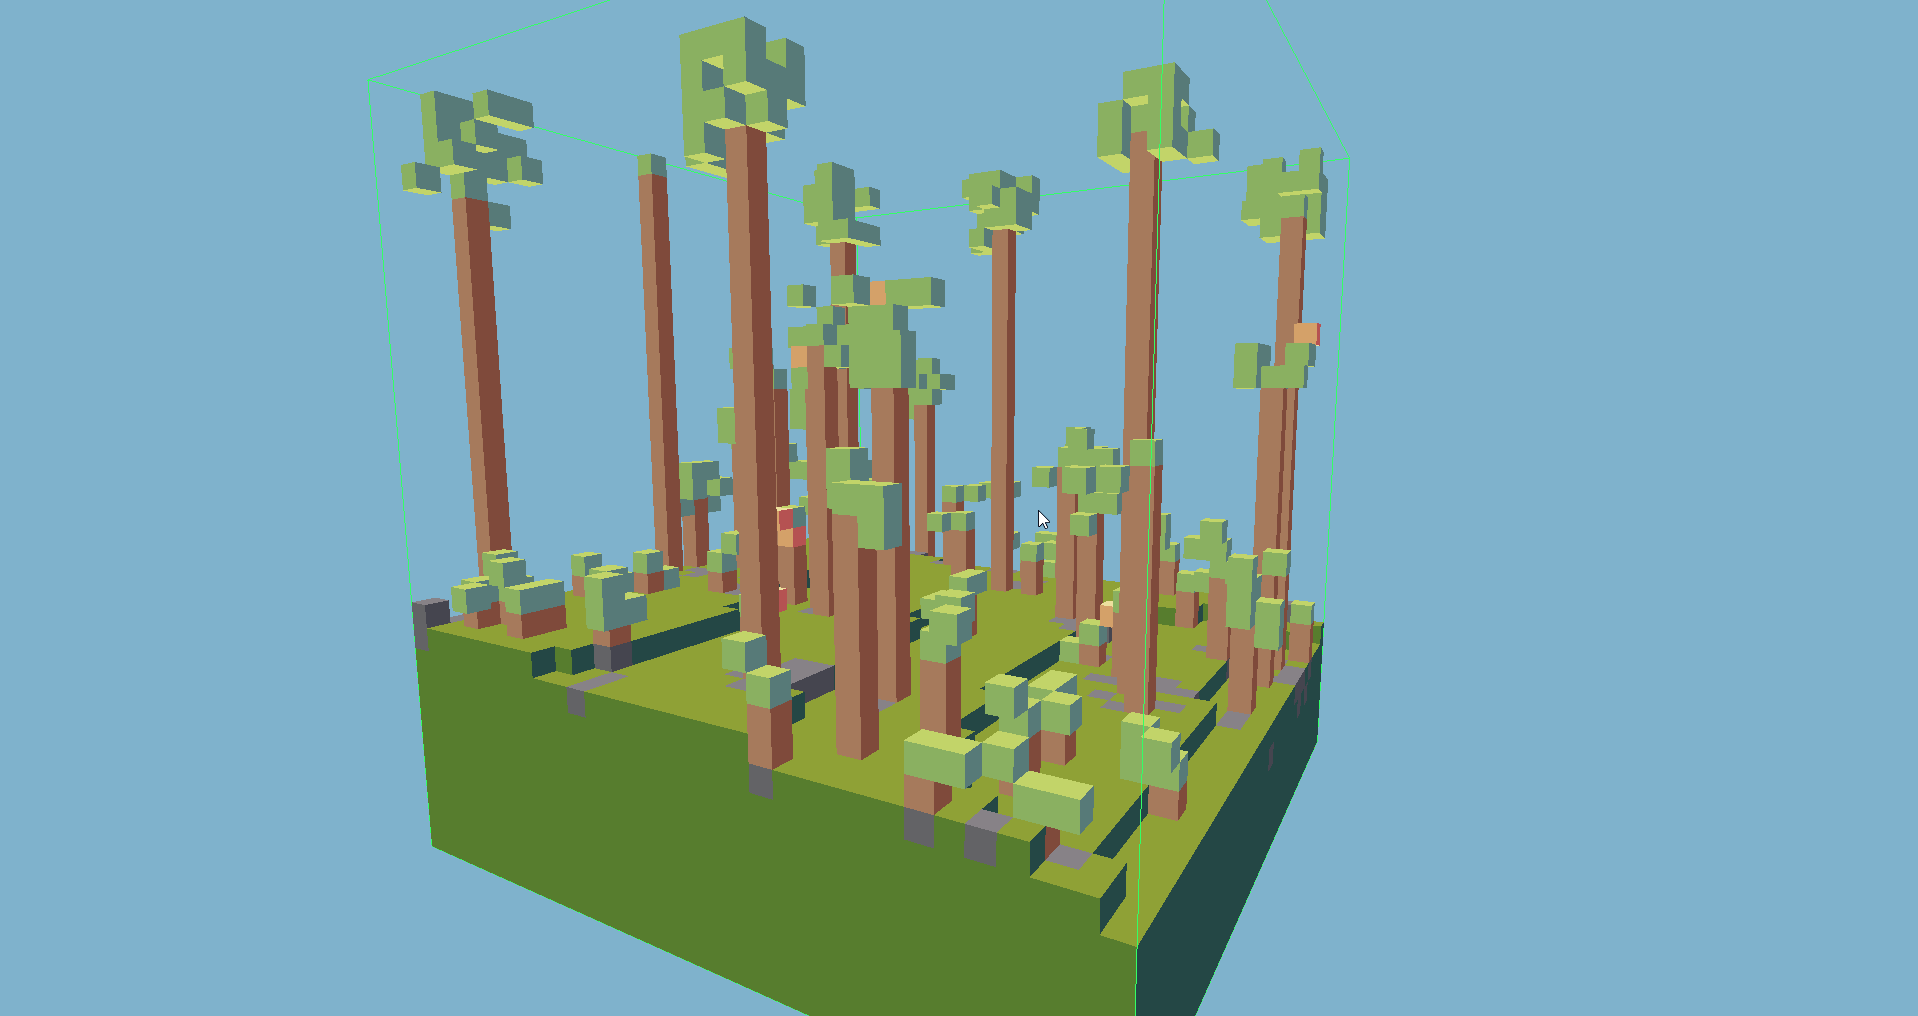
\includegraphics[width=0.7\textwidth]{res/screenshot.png}
	\caption{Snímka simulácie.}
\end{figure}

Preukázali sme, že celulárne
automaty s genetickým mechanizmom sú vhodné na modelovanie dynamického rastu
rastlín. Naše výsledky ukazujú, že použitie celulárnych automatov na simuláciu
rastlín poskytuje flexibilný a efektívny model. Rastliny sa dokážu adaptovať
na prostredie a meniť svoj rast podľa dostupnosti živín, čo pridáva prvok
prirodzenej selekcie.

Medzi silné stránky riešenia patrí modularita a
flexibilita - model možno rozšíriť o nové pravidlá rastu alebo iné prvky
simulácie (napr. vplyv podnebia); efektívne využitie zdrojov - využitie OpenGL
pre renderovanie ušetrilo CPU čas, čo umožnilo detailnejšiu simuláciu;
pozorovanie evolučných zmien - rastliny sa menia generáciami vďaka mutáciám
v genetickom kóde, čo demonštruje potenciál modelovania evolúcie.

Medzi slabiny riešenia a možnosti zlepšenia patrí obmedzená komplexnosť
genetiky - aj keď genetický kód ovplyvňuje rast, model zatiaľ neobsahuje
komplexnejšie mechanizmy; statické podmienky prostredia - simulácia zatiaľ
nezahŕňa dynamické faktory ako meniace sa počasie alebo sezónne zmeny.

Napriek týmto obmedzeniam je Botanica silným východiskovým bodom pre ďalší
výskum v oblasti simulácie rastlín a evolučných procesov v digitálnych
ekosystémoch.

\section{Závery práce}

Táto práca sa zamerala na návrh a realizáciu simulácie rastu rastlín pomocou
bunkových automatov. Náš prístup sa ukázal ako efektívny pri modelovaní
dynamických procesov rastu, avšak počas vývoja sa vyskytlo viacero výziev,
ktoré ovplyvnili priebeh implementácie. Medzi najvýznamnejšie patrila
implementácia algoritmu do jazyka C++, keďže pre 2 členov tímu tento jazyk
bol pred začatím práce neznámy a mali celkovo limitované poznatky
z programovania. Niektoré technické aspekty, najmä správa pamäte a efektívne
vykresľovanie voxelového priestoru, si vyžadovali dodatočné úpravy
a optimalizáciu. Tieto poznatky nám priniesli cenné skúsenosti, ktoré môžeme
využiť v budúcnosti.

Jedným z hlavných zistení nášho tímu bolo, že aj jednoduché pravidlá bunkových automatov
môžu viesť k vzniku komplexných a realistických štruktúr. Tento výsledok
potvrdzuje vhodnosť zvoleného prístupu a naznačuje možnosti ďalšieho rozšírenia
modelu o sofistikovanejšie faktory, ako je implementácia zvierat do systému,
zrážky alebo ročné obdobia.

Napriek uvedeným výzvam sa podarilo vytvoriť funkčný model, ktorý ponúka rôzne
možnosti konfigurácie a experimentovania s parametrami rastu. Táto práca môže
slúžiť ako základ pre ďalší výskum a aplikácie v oblastiach, hlavne v simuláciách
rastlinných systémov v počítačových hrách.


\section{Zhrnutie}

Cieľom tejto práce je navrhnutie možnej alternatívy alebo rozšírenia
ku procedurálnemu generovaniu rastlín, ktorá umožňuje rastlinám reagovať na
prostredie, v~ktorom sa nachádzajú, čím sa spestrí svet pre hráča. Táto práca
demonštruje aplikáciu, ktorá pre oživenie procedurálne
generovaného sveta využíva algoritmus simulujúci základné procesy rastlín.
Aplikácia sa skladá z troch častí: generovanie malej časti trojrozmerného
voxelového sveta pomocou Perlinovho šumu, algoritmus na simuláciu rastlín
inšpirovaným celulárnymi automatmi a~renderovanie tejto časti sveta s
využitím grafického API OpenGL.


\renewcommand\refname{Zoznam použitej literatúry}
\begin{thebibliography}{99}
	\addcontentsline{toc}{section}{\refname}

	\bibitem{Simulation of Plant Populations' Dinamics}
	Bandini, Stefania and Pavesi, Giulio,
	``A Model Based on Cellular Automata for the Simulation of the Dynamics of Plant Populations''
	(2004). International Congress on Environmental Modelling and Software. 160.

	\bibitem{Lindenmayer Systems, Fractals, and Plants}
	Prusinkiewicz, Przemyslaw and Hanan, James; Lindenmayer Systems, Fractals, and Plants;
	Springer Science \& Business Media, 2013 ; 122; ISBN - 1475714289, 9781475714289

	\bibitem{Game of Life Cellular Automata}
	Adamatzky, Andrew, ed. (2010). Game of Life Cellular Automata. Springer.
	ISBN 978-1-84996-216-2.

	\bibitem{Growth and decay in life-like cellular autometa}
	Eppstein, David. "Growth and decay in life-like cellular autometa". In Adamatzky (2010)

	\bibitem{Cellular Automata: Theory and Experiment}
	Gutowitz, Howard, ed. (1991). Cellular Automata: Theory and Experiment. MIT Press

	\bibitem{Simulation of root forms using cellular automata model}
	Winarno, Prima, Afifah;
	Simulation of root forms using cellular automata model.
	AIP Conf. Proc. 8 February 2016; 1708 (1): 070013.

\end{thebibliography}


\section{Zoznam príloh}

\begin{itemize}
	\large
	\item Príloha \textbf{A} - Snímky simulácie
	\item Príloha \textbf{B} - Botanica, zdrojový kód
	\item Príloha \textbf{C} - Manuál aplikácie Botanica
\end{itemize}

\end{document}
